\subsection{Transformation of the Notes for Sharing}

The first step of the process consists of preparing the note for publishing. In this phase all the relevant information about the note is included in the content, specifically the title, creation and last modification time, the tags and the referenced resources. This transformation is necessary, so that less information, specifically only the HTML content of the note is sent to the server, and not the entire RDF graph describing the note. Although the content is already stored as HTML, to include all the metadata about the note, it has to be enriched with RDFa before being posted to the server.

The preparation step is done on the desktop side, by the added extension to SemNotes. 
To include the referenced resources in RDFa, we need to know their server URIs. Therefore the application needs to communicate with the server to retrieve several URIs: 
\begin{itemize}
 \item the URI for the new note to be published, and 
 \item the server URI for each resource referenced by the note. 
\end{itemize}

In case the note has already been published, the user can overwrite the old post (on the Web) or create a new one. Depending on this choice, a new URI is requested from the server, or the existing one is used (that was saved in the local repository when the note was previously published). 

The referenced resources are shared by all the published notes, therefore the server must create the URI for a resource only if it has not been created before. To decide whether a local resource already has a server URI created, the list of Web aliases found for it on the desktop in the second prerequisite step of the process, is sent to the server (see JSON data in Listing \ref{lst:messagetoserver}). If a resource with a matching type and an overlapping list of aliases exists, the server reuses it, otherwise it creates a new one and saves the information about it in its own RDF repository. On the server, the URI aliases are saved as \verb|owl:sameAs| as it is customary for Linked Data. The server URIs for the note and the resources are also stored on the desktop for reuse, as \verb|pimo:hasOtherRepresentation|.
\lstset{
	caption={JSON formatted message sent to the server.}, 
	label=lst:messagetoserver,
	language=js
}
\setlength\parindent{0in}
\begin{minipage}[t]{\linewidth}
\begin{lstlisting}
{
   "id" : "",
   "resources": [
   {
      "id": "nepomuk:/res/bfcdcd1a-4898-492f-940b-4cc4c67799a7",
      "type": "mo:MusicArtist",
      "uris": [
         "http://dbpedia.org/resource/Scorpions_(band)",
         "http://musicbrainz.org/artist/c3cceeed-3332-4cf0-8c4c-bbde425147b6"
      ]
   }
   ]
}
\end{lstlisting}
\end{minipage}
\setlength\parindent{0.21in}

\lstset{
	caption={Server reply with the server URIs for the resource aliases sent.}, 
	label=lst:serverreply,
	language=js
}
\setlength\parindent{0in}
\begin{minipage}[t]{\linewidth}
\begin{lstlisting}
{
   "note":{
      "uri":"http://notes.server/note/4baccab834e20",
      "resources":[
         {
            "local":"nepomuk:/res/bfcdcd1a-4898-492f-940b-4cc4c67799a7",
            "uri":"http://notes.server/resource/4bacca84ca8bb"
         }
      ]
   }
}
\end{lstlisting}
\end{minipage}
\setlength\parindent{0.21in}

In the case when no Web aliases are found for a desktop resource that is related to a note, and thus the list of aliases sent to the server is empty, a new resource is created on the server with the specified type, but without any information attached to it. The server URI is saved on the desktop as \verb|pimo:hasOtherRepresentation| of the resource, and will be available for reuse when other notes related to the same object are published by the same user. However, this resource will not be shared between notes published by different users. If at a later stage a Web alias is found for the desktop resource, it will be added to the resource already created on the server, thus enabling it to be linked to by multiple users.

The communication between SemNotes and the server is done with a single REST call, in order to minimise network delays. The reply contains the newly created URI for the note, if one was required, as well as a list of server URIs for the resources (see JSON data in Listing \ref{lst:serverreply}). The communication between the desktop side and the server is shown in Figure \ref{fig:semblogsequencediag}. 

Using the information received from the server, the note content is enriched with RDFa. The metadata about the note, like type, creation and last modification times and the tags, is added in \verb|meta| tags in the \verb|head| of the HTML page. RDFa is added to the \verb|title| tag and in the \verb|body|, to the links. Listing \ref{lst:rdfa} shows the content of a note prepared for publishing.

\begin{figure}[htb]
  \begin{center}
    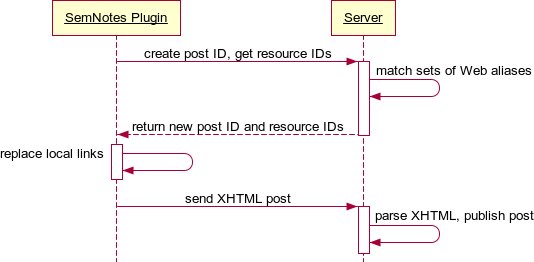
\includegraphics[width=0.85\linewidth]{chapters/core/img/sequencediagram}
    \caption{Sequence diagram for the communication with the server.}
    \label{fig:semblogsequencediag}
  \end{center}
\end{figure}

\lstset{
	caption={RDFa-annotated XHTML content of note.}, 
	label=lst:rdfa,
	language=htmlrdfa
}
\setlength\parindent{0in}
\begin{minipage}[t]{\linewidth}
\begin{lstlisting}
<!DOCTYPE html PUBLIC '-//W3C//DTD XHTML RDFa 1.0//EN' 
                      'http://www.w3.org/MarkUp/DTD/xhtml-rdfa-1.dtd'>
<html about="http://notes.server/note/4baccab834e20">
    <head>
        <meta content="sioc:Post" property="rdf:type"/>
        <meta rel="sioc:topic" href="http://notes.server/tag/concert"/>
        <title property="dc:title">concert sunday</title>
    </head>
    <body>
        <a rel="sioc:is_related"
             href="http://notes.server/resource/4bacca84ca8bb">scorpions</a> concert on sunday was great ...
    </body>
</html>
\end{lstlisting}
\end{minipage}
\setlength\parindent{0.21in}
